\begin{figure*}[h!]
\centering
%
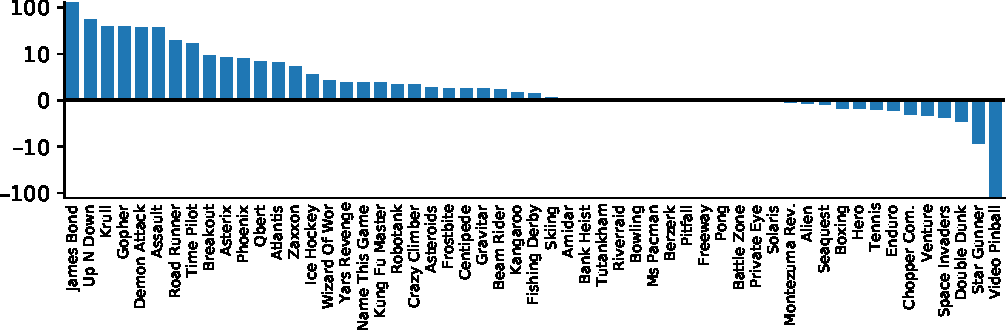
\includegraphics[width=\textwidth]{vs/dreamerv2-vs-iqn}
\vspace*{-32.5ex}\begin{center}DreamerV2 vs IQN\end{center}\vspace*{32.5ex}
\vspace*{-5ex}
%
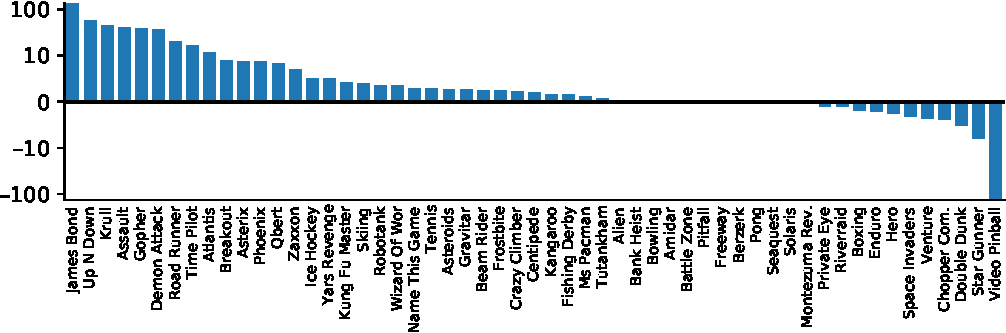
\includegraphics[width=\textwidth]{vs/dreamerv2-vs-rainbow}
\vspace*{-32.5ex}\begin{center}DreamerV2 vs Rainbow\end{center}\vspace*{32.5ex}
\vspace*{-5ex}
%
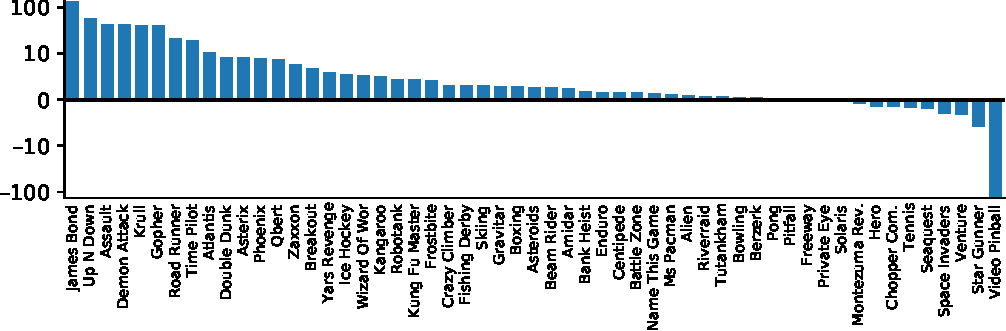
\includegraphics[width=\textwidth]{vs/dreamerv2-vs-c51}
\vspace*{-32.5ex}\begin{center}DreamerV2 vs C51\end{center}\vspace*{32.5ex}
\vspace*{-5ex}
%
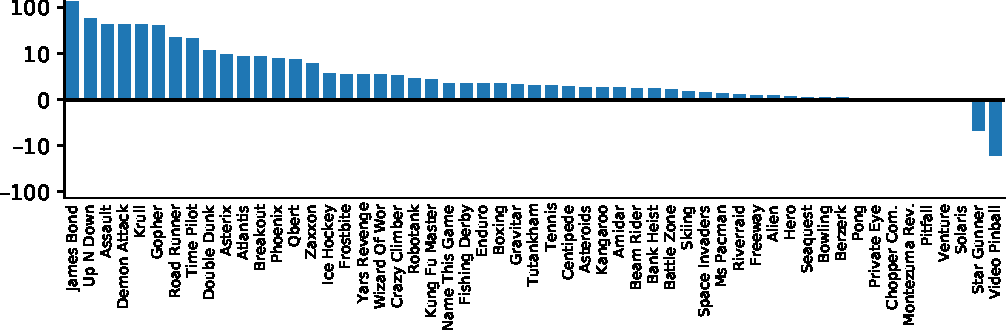
\includegraphics[width=\textwidth]{vs/dreamerv2-vs-dqn}
\vspace*{-32.5ex}\begin{center}DreamerV2 vs DQN\end{center}\vspace*{32.5ex}
\vspace*{-6ex}
%
\caption{Atari agent comparison. The bars show the difference in gamer normalized scores at 200M steps. DreamerV2 outperforms the four model-free algorithms IQN, Rainbow, C51, and DQN while learning behaviors purely by planning within a separately learned world model. DreamerV2 achieves higher or similar performance on all tasks besides Video Pinball, where we hypothesize that the reconstruction loss does not focus on the ball that makes up only one pixel on the screen.}
\label{fig:vs}
\end{figure*}
